% \begin{document}
\chapter{Astrazione sul controllo: sottoprogrammi ed eccezioni}

A cosa servono gli array? Il linguaggio assembly non ce li ha, ma riesce comunque a svolgere tutto quello che possono fare. Sono quindi un'\textit{astrazione} che rende la vita dei programmatori piu' facile. Questo e' l'obbiettivo dei linguaggi di programmazione di alto livello, che astrae sul controllo e sui dati. 

L'astrazione, quindi, consiste nell'indentificare proprietà importanti di cosa si vuole descrivere, concentrarsi su quelle e ignorare le altre. Che cosa ignorare e cosa no dipende dallo scopo del progetto

I linguaggi di programmazione (oltre al fatto che essi stessi sono astrazioni più sono ad alto livello) forniscono strumenti per implementare astrazioni e modelli astratti, questi sono chiamati, appunto, \textbf{astrazioni sul controllo e sui dati}. Adesso diamo una definizionzioncina

\dfn{astrazione sul controllo}{
    Si definisce \textbf{astrazione del controllo} una serie di istruzioni per svolgere un compito a prescindere dal contesto in cui questo opera, specificandone modalità e fine 
}

Queste astrazioni sono ad esempio funzioni o blocchi. Tra le proprietà più importanti di questi costrutti è che ogni componente fornisce servizi al suo ambiente, nascondendo i dettagli interni necessari a produrlo

Un meccanismo fondamentale con cui si può definire come ogni sottoprogramma (funzione) comunica con il col programma principale \texttt{main} è attraverso i parametri o un'ambiente globale (da preferire i primi perché quest'ultimo rende nulla l'astrazione)

\section{parametri}

Introduciamo due definizioni terminologiche:
\dfn{Parametro formale}{
    Un parametro formale è una variabile utilizzata nella definizione di un sottoprogramma, che viene sostituita dal valore o riferimento del parametro attuale quando il sottoprogramma viene chiamato.
}

Pertanto si trova nella dichiarazione/definizione: \texttt{int f (int }\textbf{n}\texttt{){return n+1;}}

    \dfn{Parametro attuale}{
        Un parametro attuale è il valore o riferimento passato a un sottoprogramma quando viene chiamato. Questo valore o riferimento sostituisce il parametro formale nella definizione del sottoprogramma.
    }

Ad esempio, nell'espressione \texttt{f(5)}, il valore \texttt{5} è il parametro attuale che sostituisce il parametro formale \texttt{n} nella definizione del sottoprogramma \texttt{f}.

\dfn{Pragramtica}{
    La pragramtica rappresenta il flusso di informazioni tra chiamante e chaiamto
}

Rappresentiamo il chiamate con \texttt{main} e il chiamato \texttt{proc}, questi sono i possibili di informazioni tra i comuniscanti:
\begin{itemize}
    \item \texttt{main}$\to$\texttt{proc}, es. \texttt{x=f(y+1)}
    \item \texttt{proc}$\to$\texttt{main}, es. \texttt{procedure Uno (var y:integer); begin y:=1 end;}
    \item \texttt{proc}$\leftrightarrow$\texttt{main}, es. \texttt{procedure Succ (var y:integer); begin y:=y+1 end;}
\end{itemize}


\ex{Una funzione comunica col chiamante}{
    Valore restituito
    
    \texttt{int f(){return 1;}}
}

\subsection{Modalità di passaggio dei parametri}
Vi sono due modi principali per passare i parametri ai sottoprogrammi:

\begin{itemize}
    \item \textbf{Passaggio per valore}: In questo caso, il valore del parametro attuale viene copiato nel parametro formale del sottoprogramma. Le modifiche apportate al parametro formale all'interno del sottoprogramma non influenzano il parametro attuale.
    
    La pragramtica è \texttt{main $\to$ proc}

    \ex{Esempio di passaggio per valore}{
        \texttt{void increment(int n) \{ n = n + 1; \}}
        
        \texttt{int main() \{ int x = 5; increment(x); \}}
        
        In questo esempio, il valore di \texttt{x} non cambia dopo la chiamata a \texttt{increment}.
    }

    \item \textbf{Passaggio per riferimento}: In questo caso, il parametro formale del sottoprogramma diventa un riferimento al parametro attuale. Le modifiche apportate al parametro formale all'interno del sottoprogramma influenzano direttamente il parametro attuale
    
    La pragramtica è \texttt{main $\leftrightarrow$ proc}
    
    \ex{Esempio di passaggio per riferimento}{
        \texttt{void increment(int \&n) \{ n = n + 1; \}}
        
        \texttt{int main() \{ int x = 5; increment(x); \}}
        
        In questo esempio, il valore di \texttt{x} cambia a 6 dopo la chiamata a \texttt{increment}.
    }
\end{itemize}

\subsubsection{Passaggio per valore}
Si prenda come esempio il seguente codice

\begin{lstlisting}[language=C]
    void foo (int x) { x = x+1; }
    {...}
    y = 1;
    foo(y+1);
\end{lstlisting}

In questo caso il parametro formale \texttt{x}, mentre quello attuale è \texttt{y}. Alla chiamata di \texttt{foo}, viene valutato \texttt{y+1} e assegnato al formale{x}. Ovviamente non vi sarà nessun legame tra \texttt{x} e \texttt{y} e alla fine della computazione \texttt{x} verrà deallocata e distrutta.

Tuttavia si ha che nel record  di attivazione di \texttt{foo}, appena viene eseguita la funzione, vine ecreata una copia di \texttt{y} per \texttt{x}. La cosa è influente dato che \texttt{x} è un intero, ma potrebbe essere estremamente costoso per parametri attuali di grandi dimensioni, si pensi ad un array di 1000 elementi

\subsubsection{Passaggio per riferimento}
Si prenda come esempio il seguente codice

\begin{lstlisting}[language=C]
    void foo (reference int x){ x = x+1;}
    ...
    y = 1;
    foo(y);
\end{lstlisting}

In questo caso, nella funzione viene passato un riferimento, ovvero un puntatore a un intero. Pertanto, qualsiasi modifica apportata al parametro formale \texttt{x} all'interno della funzione \texttt{foo} influenzerà direttamente il parametro attuale \texttt{y}. Tra la variabile \texttt{x} e \texttt{y} si verifica il cosidetto \textit{aliasing} alla stessa cella

Questo metodo è efficiente in termini di memoria, poiché non viene creata una copia del parametro attuale. Tuttavia, bisogna fare attenzione alle modifiche non intenzionali ai parametri attuali, poiché queste possono portare a effetti collaterali indesiderati

\subsubsection{Passaggio per costante}

Il passaggio per costante è una variante del passaggio per valore, tuttavia viene garantito che nella procedura non è permessa la modifica del parametro formale

\begin{lstlisting}[style=cstyle]
void foo (final int x){
  // qui x non puo' essere modificato
}
\end{lstlisting}

Se l'oggetto passato e' di grandi dimensioni, il compiler puo' evitare di fare la copia usando il passaggio a riferimento, mantenendo sempre la semantica del passaggio per valore.

\subsubsection{Passaggio per Risultato}

\begin{lstlisting}[language=C]
    void foo (result int x) {x = 8;}
    ...
    y = 1;
    foo(y);
\end{lstlisting}

Il passaggio per risultato è la tecnica \textit{complementare} al passaggio per valore. In questo caso, il parametro formale viene utilizzato per restituire un valore al termine dell'esecuzione del sottoprogramma

Al momento della chiamata e della computazione (all'interno del corpo di \texttt{foo}) non vi sarà alcun legame tra \texttt{x} e \texttt{y}, ma al ritorno di \texttt{foo} verrà fatta una copia di del formale sull'attuale \texttt{y=x}
La pragramtica sarà dunque: \texttt{proc $\to$ main}

\subsubsection{Passaggio per valore risultato}
È un mix tra il passaggio per risultato e per valore, pertanto verrà fatta una copia dall'attuale a formale all'inizio e una copia dal formale all'attuale alla fine e, dato che non vi è alcun riferimento, non vi è alcun legame tra il formale e l'attuale durante la computazione dei dati nel corpo della funzione

Pragmaticamente: \texttt{main$\leftrightarrow$proc}


Si noti che il passaggio valore-risultato $\neq$ riferimento, ad esempio in questo codice:

\begin{lstlisting}[language=C]
    void foo (int x, int y, int z) {
        x = 2;
        y = 2;
        x = 4;
        if (x == y) z = 1;
    }
    int a = 3;
    int b = 0;
    foo(a,a,b);
\end{lstlisting}

Per valore risultato il valore delle variabili istruzione per istruzione è

\begin{center}
    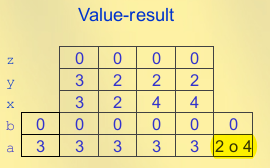
\includegraphics{img/valueresult.png}
\end{center}

Mentre per riferimento
\begin{center}
    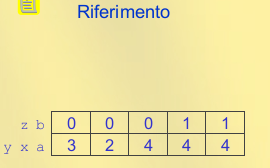
\includegraphics{img/riferimento.png}
\end{center}



\subsubsection{Morale}
Il passaggio per valore ha come pro:
\begin{itemize}
    \item Semantica semplice: il corpo non ha necessità di conoscere come la procedura verrà chiamatà
    \item trasparenza referenziale: ovvero la proprietà di un'espressione che garantisce che verrà restituito sempre lo stesso risultato ogni qualvalto il gli verrà fornito lo stesso imput indipendentemente dal contesto
    \item implementazione abbastanza semplice
\end{itemize}
e come contro un costo potenzialmente alto per la copia del parametro attuale.

Invece il passaggio per riferimento ha come pro:
\begin{itemize}
    \item implementazione semplice
    \item efficienza nel passaggio da parametro attuale a formale
\end{itemize}

E come contro una semantica complessa a causa dell'aliasing
\subsubsection{Passaggio per nome}

Il passaggio per nome è una modalità di passaggio parametri introdotta da Algol negli anni 60 che vede la chiamata come una \textit{macro espansione} ovvero un meccanismo dove la semantica di una chiamata di funzione è definita in modo \textbf{prescrittivo} e consiste nell'esecuzione del corpo come se fosse testualmente presente nel chiamante, anche la gestione dei parametri segue lo stesso principio, ovvero il corpo della procedura viene eseguito dopo che i parametri attuali sono stati sostituiti testualmente al posto dei parametri formali, quindi quest'ultimi vengono valutati dopo questo passaggio. 

Più in particolare il passaggio per nome segue la cosiddetta \textit{regola della copia}: una chiamata alla procedura P è la stessa cosa che eseguire il corpo di P dopo aver sostituito i parametri attuali al posto dei parametri formali.

Si noti il seguente codice:

\begin{lstlisting}[language=C]
    int y;
    void foo (name int x) {x= x + 1; }
    ...
    y = 1;
    foo(y);    
\end{lstlisting}

In questo caso dopo la chiamata \texttt{foo(y)} viene inserito il corpo della funzione nel \texttt{main}  cambiando il parametro formale con quello attuale, quindi \texttt{y=y+1}. Tuttavia questa regola per come è definita nasconde una criticità, infatti se nel corpo della funzione è presente un nome \texttt{y} potrebbe provocare un conflitto, si noti questo codice:

\begin{lstlisting}[language=C]
    int y;
    void fie (name int x){
    int y;
    x = x + 1; y = 0;
    }
    ...
    y = 1;
    fie(y);
\end{lstlisting}

Dopo la della chiamata verrà eseguita la macro espansione sostituendo il parametro formale con quello attuale:
\begin{lstlisting}[language=C]
    int y;
    y = y+1;
    y =0;
\end{lstlisting}

Tuttavia all'interno di \texttt{fie} vi erano due variabili erano diverse che abbiamo reso uguali perché il nome di \texttt{y} all'interno di \texttt{fie} è uguale al parametro attuale, provocando così un conflitto se si esegue il programma con scope statico. 

Per ovviare a questo problema viene passato, ai vari paramatri, una coppia \texttt{<exp, amb>} detta \textit{closure}, dove:
\begin{itemize}
    \item \texttt{exp}: è il parametro attuale (testo, non valutato)
    \item \texttt{amb}: è l’ambiente di valutazione (in scoping statico)
\end{itemize}

Si prenda come esempio il seguente codice:
\begin{lstlisting}[language=C]
    int y;
    void fie (int x ){
        int y;
        x = x + 1; y = 0;
    }
    ...
    y = 1;
    fie(y);
\end{lstlisting}

Quando viene eseguita la macro-espansione si avra che \texttt{x$\to$<y, int y;>} dove l'ambiente non è altro che la dichiarazione della variabile in riga 1, gg. Si ha, quindi, che \textit{ogni volta che il formale è usato, exp è valutata in amb}

La pragmatica in questo è \texttt{main$\leftrightarrow$proc}, inoltre si tratta di una pratica costosa infatti

\begin{itemize}
    \item \textbf{vi è il passaggio di una strutta complessa} (soprattutto l'ambiente)
    \item \textbf{è prevista una rivalutazione ripetuta del parametro}, infatti differenza del passaggio per valore, in cui il parametro viene valutato una sola volta prima di entrare nella funzione, nel passaggio per nome il parametro viene rivalutato ogni volta che viene usato nel corpo della funzione
\end{itemize}

Per implementare il passaggio per nome, la coppia closure è formata, dal lato pratico, da:
\begin{itemize}
    \item un puntatore al testo di \texttt{exp}
    \item un puntatore di catena statica (sullo stack) al record di attivazione del blocco di chiamata
\end{itemize}
\section{Funzioni di ordine superiore}
Alcuni linguaggi di programmazione consenstono di passare passare \textbf{funzioni come argomenti di altre funzioni} o  \textbf{restituire funzioni come risultato di una funzione}:

\dfn{Funzione di ordine superiore}{
  Funzione che accetta una funzione come parametro o che restituisce una funzione come risultato.
}
è quindi lecito chiedersi come viene gestito lo scope in questi casi

\subsection{Funzione come argomento}
Vediamo un esempio:
\begin{lstlisting}[language = C]
  A:{
    int x = 1;
    int f (int y){
      return x+y; // Quale "x"?
    }
    void g(int h(int b)){
      int x = 2;
      return h(3) + x;
    }
    ...
    B:{
      int x = 4;
      int z = g(f)
    }
  }
\end{lstlisting}
Notare che f utilizza una variabile non-locale x, che e' stata dichiarata piu' volte: nel blocco A, B e nella funzione g. Dobbiamo quindi capire in quale ambiente risolverla, proviamo ad applicare le regole di scope che abbiamo visto fin'ora:
\begin{itemize}
    \item se lo scope è statico: si usa \texttt{x} definita nel punto in cui \texttt{f} è stata dichiarata \texttt{(x=1)}
    \item Se lo scope è dinamico: si potrebbe usare sia la \texttt{x} della chiamata \texttt{x=4}, sia la \texttt{x} di \texttt{g} (\texttt{x=2})
\end{itemize}

L'incertezza su quale ambiente non-locale scegliere e' dovuta dal fatto che e' possibile immaginare due implementazioni diverse della chiamata di una funzione passata come parametro (f) tramite il parametro formale (h):

\begin{itemize}
  \item La chiamata della funzione passata avviene nel blocco della funzione di ordine superiore (la chiamata h(3) chiama la funzione f all'interno di g)
  \item La chiamata della funzione passata avviane nel blocco dove viene creato il legame fra parametro formale e attuale (la chiamata h(3) chiama la funzione f all'interno del blocco B)
\end{itemize}

Quindi notiamo che le regole di scope non sono abbastanza specifiche per determinare l'ambiente da utilizzare, dato che non e' chiaro da quale blocco si vuole che avvenga la chiamata di f (in questo caso lo scope statico ha solo un'opzione, ma vedremo che non e' sempre cosi'). Ci servono quindi delle ulteriori regole specifiche alle funzioni parametro, dette regole di \textit{binding}:

\dfn{Binding}{
  Data una funzione di ordine superiore g che ammette una funzione parametro f, in base al blocco dal quale vogliamo che f venga chiamato quando chiamiamo il parametro formale associato h, abbiamo due casi:
  \begin{itemize}
  \item \textit{Deep binding}, se la chiamata avviene nel blocco attivo nel momento in cui e' stato instaurato il legame fra parametro formale e attuale.
  \item \textit{Shallow binding}, se la chiamata avviene nel blocco attivo nel momento in qui viene chiamato il parametro formale.
  \end{itemize}
}

Quindi, applicando cio' all'esempio di prima:
\begin{itemize}
  \item Usando deep binding, si simula la chiamata di f dal blocco B, quindi con scope statico x = 1 e con scope dinamico x = 4.
  \item Usando shallow binding, f viene chiamata dalla funzione g, quindi se si usa scope statico abbiamo comunque x = 1, ma con scope dinamico x = 2.
\end{itemize}

Vediamo in specifico l'implementazione delle due regole di binding applicate in linguaggi con scope dinamico e statico:
\subsubsection{Binding con scope dinamico}
Consideriamo prima il caso di un linguaggio con scope dinamico e shallow binding. Per definizione di shallow binding, vogliamo chiamare la funzione parametro f all'interno del corpo della funzione g. Per le regole dello scope dinamico, dobbiamo risolvere le variabili non-locali nell'ambiente immediatamente precedente alla chiamata, che quindi corrisponde all'ultimo record di attivazione sulla pila (quello di g). In questo caso quindi basta la normale implementazione di scope dinamico.

\begin{center}
  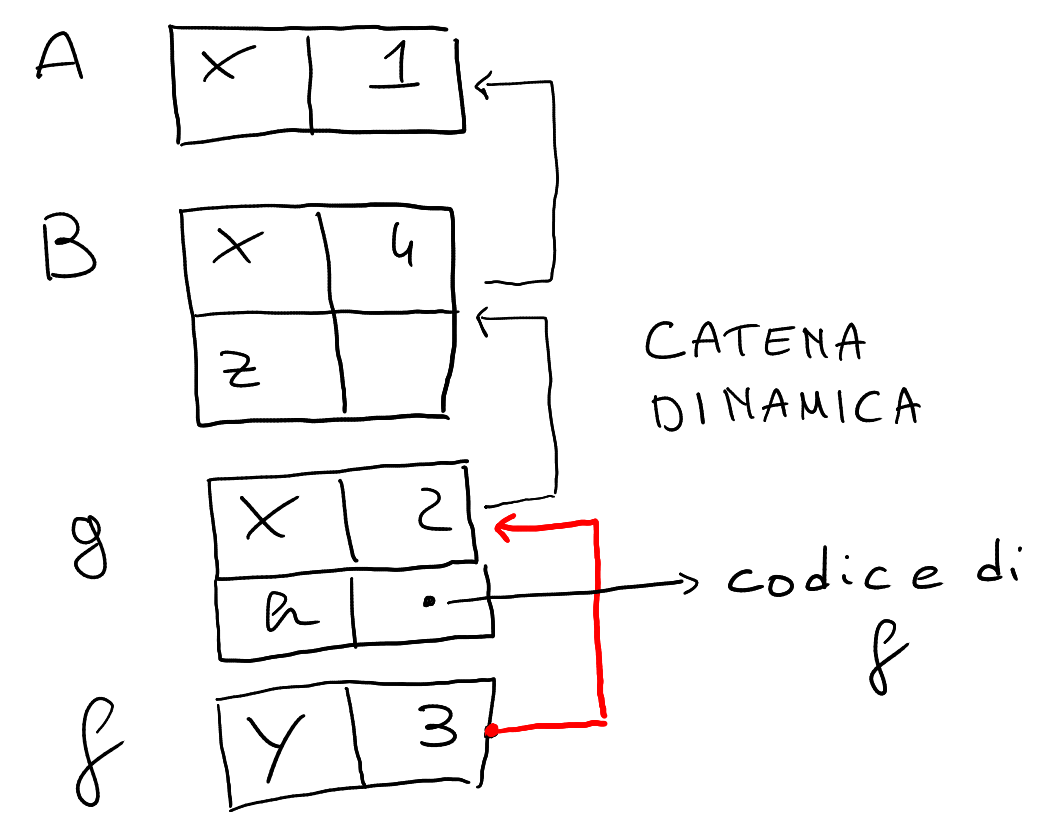
\includegraphics[width=0.3\textwidth]{img/2025-03-21-20-26-21.png}
\end{center}
\nt{
  Ovviamemte puo' anche essere implementato lo scope dinamico con A-list o CRT.
}

Nel caso di deep binding con scope dinamico, ci serve l''ambiente del blocco attivo al momento del legame fra la funzione e il parametro formale. Ma in questo caso, l'RdA di questo blocco (che nell' esempio e' B) non sara' direttamente sotto a quello della funzione f quando viene chiamata, dato che ci sara' sicuramente almeno il frame della funzione di ordine superiore. Dobbiamo quindi passare un puntatore a questo ambiente insieme alla funzione. Tale struttura viene chiamata \textit{closure}, ovvero l'accoppiata $\langle$\texttt{f, amb}$\rangle$, dove:

\begin{itemize}
    \item \texttt{f} è il puntatore alla funzione che vogliamo passare
    \item \texttt{amb} è il puntatore all'ambiente non-locale in cui è da valutare il corpo della funzione f
\end{itemize}

\begin{center}
  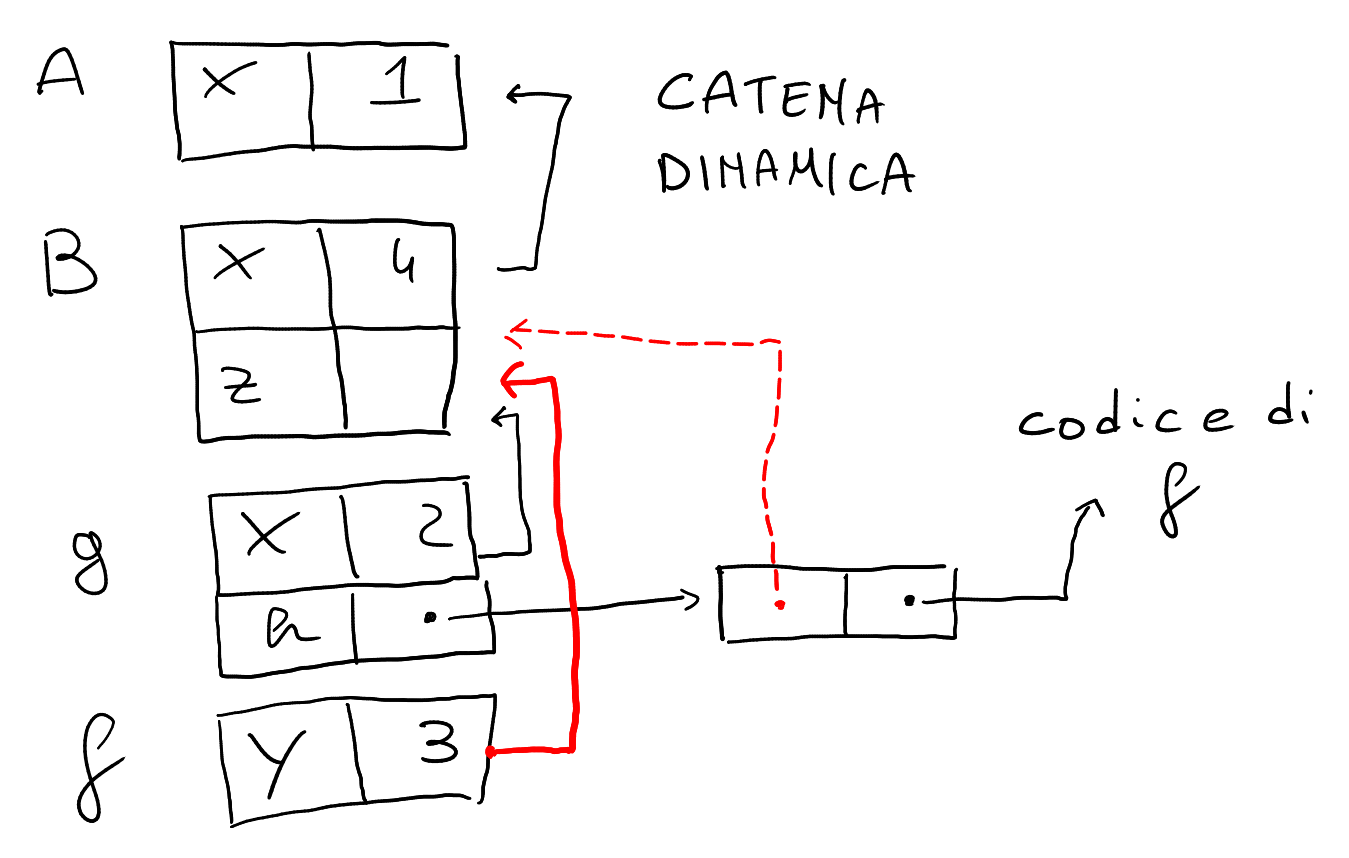
\includegraphics[width=0.3\textwidth]{img/2025-03-21-20-30-20.png}
\end{center}

\subsubsection{Binding con scope statico}

Anche nel caso generale dello scope statico e' necessario usare una closure per poter passare alla funzione di ordine superiore anche il puntatore di catena statica, che puo' essere calcolata al momento del legame fra funzione e parametro formale, come abbiamo visto studiando l'implementazione dello scope statico (\ref{calcoloCatenaStatica}).

\begin{center}
  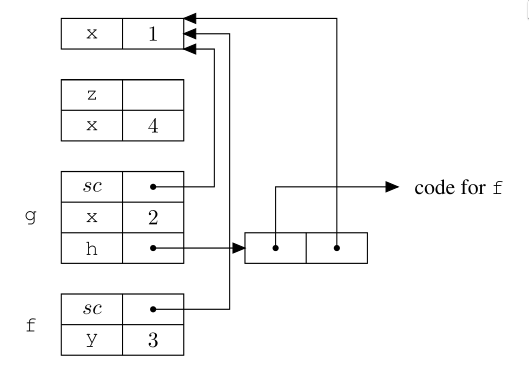
\includegraphics[width=0.3\textwidth]{img/2025-03-21-20-10-23.png}
\end{center}

Puo' sembrare che le regole di scope statico siano rigide e che non servano le regole di binding per distinguere vari casi. In effetti per la maggior parte delle situazioni e' cosi, ma ci possono essere discussioni per quanto riguarda un caso specifico con funzioni ricorsive. Vediamo un esempio:

\begin{lstlisting}[language=C]
  A:{
    void foo(int f(), int x){
      int fie(){
        return x;
      }
      int z;
      if (x==0) z = f();
      else foo(fie, 0);
    }
    int g(){
      return 1;
    }
    foo(g,1);
  }
\end{lstlisting}

Il problema in questo caso e' che la funzione fie e' definita in due istanze diverse della funzione foo, alle quali sono associati due ambienti diversi: nel primo x = 1, nel secondo x = 0. Dato che possono essere considerate valide entrambi per le regole di scope, bisogna utilizzare le regole di binding. Usando shallow binding, consideriamo la definizione piu' vicina temporalmente; usando deep binding, scegliamo l'ambiente attivo al momento della prima definizione di fie.

\begin{center}
  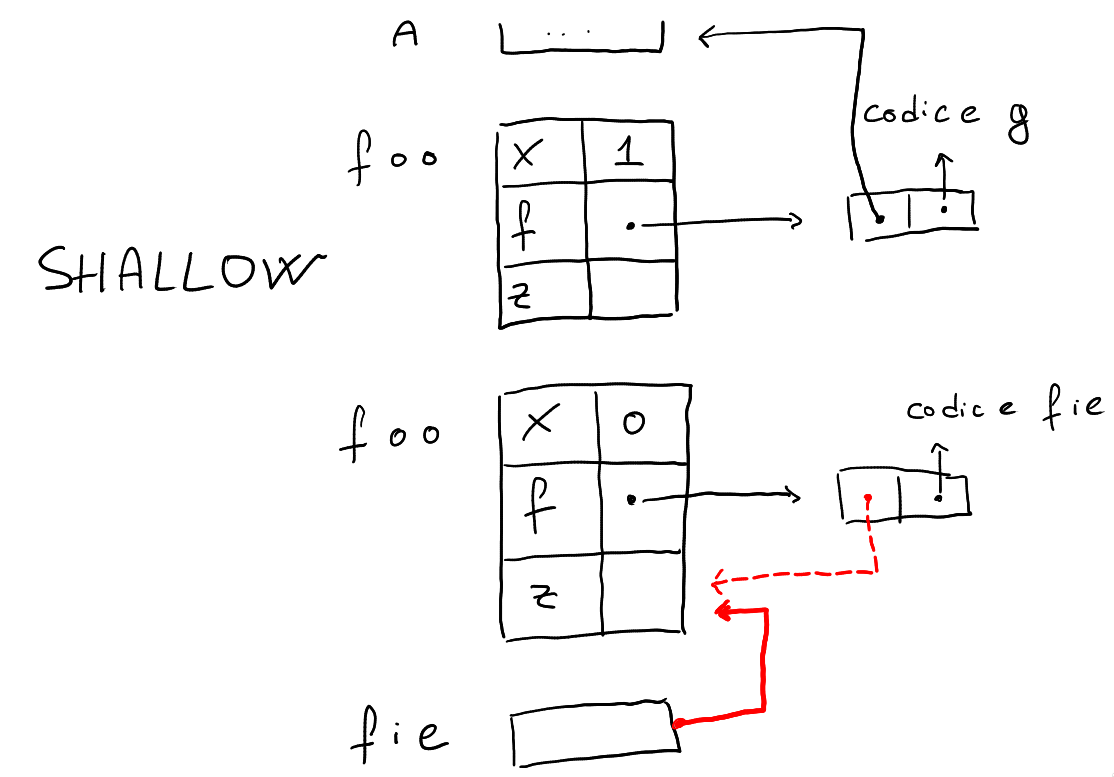
\includegraphics[width=0.4\textwidth]{img/2025-03-21-20-41-11.png}
  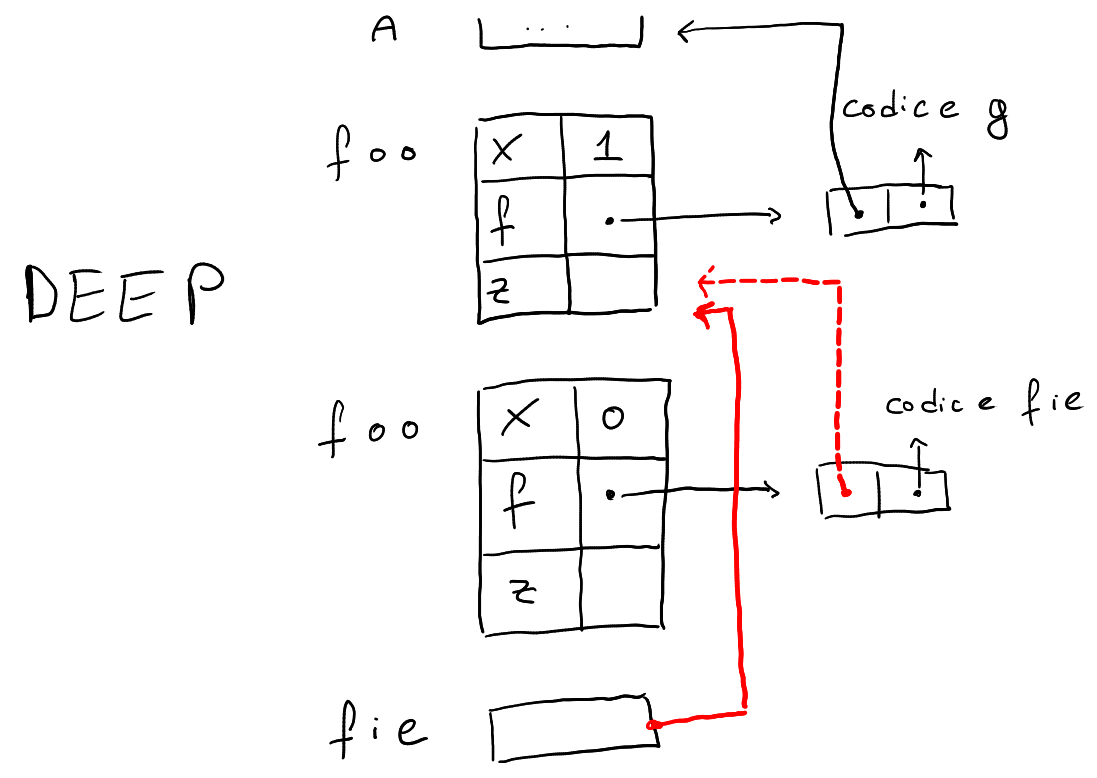
\includegraphics[width=0.4\textwidth]{img/2025-03-21-20-42-39.png}
\end{center}

% \end{document}
